\section{Introduction}
\begin{frame}
	\frametitle{Basic 'Mesh' Terminology}
  \begin{itemize}
		\item \keyword{Mesh Generation} (\keyword{Meshing}) is the act of creating a mesh for a computing task
		\item Generally a \keyword{Mesh} is a discretized representation of a geometry 
		\item Meshes are used in FEM, FV, FD, Physics Simulators (Rigid or Soft Bodies), CAD, Rendering, 3D Printing,...
		\item Mesh Generation software is often specialized for a certain target application ($\uparrow$)
		\item Larger software packages often have mesh generation software included as a component of the package
		\item Meshes used for computational tasks need to fulfill certain \keyword{quality criteria}
		\item \keyword{Quality criteria} are checked before use to prevent unnecessary failure and remeshing
		\item \keyword{Mesh Data Structures}, \keyword{Mesh Formats} and \keyword{Mesh Conversion} are essential components of the meshing workflow
  \end{itemize}	
\end{frame}

\begin{frame}
	\frametitle{Mesh Generation}
  \begin{itemize}
		\item Mesh Generation is a huge/important aspect of simulation (for mesh-based methods of course)
		\item Manual, automatic and hybrid (combination of manual + automatic) mesh generation methods
		\item Computational domains have different components that can be meshed differently
		\item Meshing of inflow, outflow, wall, embedded geometry or other special function components of the domain
		\item Surface meshes (usually surface triangulations) are frequently used to simulate flow around objects
		\item Create a mesh that fulfills the quality criteria for the designated computation task
		\item Involves scientific disciplines such as computational geometry, differential geometry, geometric modeling, optimization, etc.
  \end{itemize}	
\end{frame}

\begin{frame}
	\frametitle{Mesh Nomenclature}
  \begin{itemize}
		\item Focus on 2D Meshes, 3D Surface/Volume meshes
		\item Basic topological terminology and theory of meshes in the works of Kinsey \cite{kinsey1993topology} and 
Edelsbrunner\cite{Edelsbrunner:2006:GTM:1137760}.		
  \end{itemize}		
  \begin{block}{Definition: Mesh or Cell Complex}
  A mesh $\mathcal M$ is composed of a finite number of $n$-dimensional cells: 
	\begin{align*}
   \mathcal M =\{\omega : \omega \text{ is a element}\}.  
  \end{align*}
  \end{block}	
  \begin{itemize}
		\item \keyword{Cell Complex} is a common alternative term for mesh in literature
		\item Term is used computational geometry package \keyword{CGAL} and implemented as a data structure
  \end{itemize}			
\end{frame}

\begin{frame}
  \frametitle{Cell Complex Example}
	\begin{block}{Hexahedron Example}
   The hexahedron is composed of one 3-dimensional element/cell, the 3-dimensional cell is composed of six 2-dimensional cells, the facets. The facets are
	 composed of the 1-cells called edges/segments describing their boundaries. The endpoints of the edges are the eight 0-dimensional cells, the vertices.
	\end{block}
    \begin{center}
      \includegraphics[width=0.4\textwidth]{screenshots/hexa-cell2.png}
    \end{center}			
\end{frame}

\begin{frame}
  \frametitle{Dimension of a Cell Complex}
 	\begin{block}{Dimension of a Cell Complex}
	The dimension of a mesh is equal to the highest cell dimension in the mesh.
   A cell of a mesh is the mesh component the inner of which is homeomorphic to the inner set of an $n$-dimensional disk.  
	\end{block}
  \begin{itemize}
		\item The boundary of a cell is composed of cells of lower dimension, these lower dimensional cell boundaries are
 called \keyword{faces} or \keyword{facets}.
		\item For these relationship between faces and cells we can also use the notation $\sigma < \tau$ to indicate that $\sigma$ is a face of cell $\tau$.
		\item A polyhedron for example is a cell that is composed of polygonal faces(two-dimensional cells), edges (one-dimensional cells) and vertices (zero-dimensional cells).
  \end{itemize}	
\end{frame}

\begin{frame}
  \frametitle{Structure of a Cell Complex}
In order to construct a mesh we combine and connect cells of equal dimension: vertices are connected to vertices and edges are connected to \keyword{adjacent} edges. 
 	\begin{block}{Dimension of a Cell Complex}
By $|\mathcal M|$ we refer to the set of points of mesh $\mathcal M$:	
\begin{align*}
  |\mathcal M|=\{\vec{x} : \vec{x} \in \sigma \in \mathcal M, \text{$\sigma$ is a cell in $\mathcal M$.}\}  
\end{align*}
	\end{block}
  \begin{itemize}
		\item $|\mathcal M|$ is also called the underlying space of $\mathcal M$
		\item For every vertex in $|\mathcal M|$ a defined neighborhood relationship has to exist
		\item Neighborhood in a 2-cell complex:
		\begin{itemize}
			\item Vertex neighborhoods over edge connections
			\item Facet neighborhood over edges			
			\item Facet neighborhood over vertices
			\item ...									
		\end{itemize}				
  \end{itemize}		
\end{frame}

\begin{frame}
  \frametitle{Neighborhoods/Connectivity in a Cell Complex}
		\begin{itemize}
			\item For vertex $\vec{v}$ inside of a polygon, the neighborhood of $\vec{v}$ is an arbitrary disk that is entirely located in the inside 
of the polygon. 
			\item If the vertex $\vec{v}$ is on an edge $\vec{e}$ that was contructed by unification of edges $\vec{e}_0,\dots,\vec{e}_n$ then the corresponding vertex $\vec{v}$ has to be present on every edge $\vec{e}_i$.
			\item Facet neighborhood over vertices
			\item The unification of half-disk neighborhoods of the vertices $\vec{v}_0,\dots,\vec{v}_n$ leads to the neighbor relationship that is
depicted in figure \ref{fig:mesh-neighborhood}.
			\item When $\vec{v}$ is contructed from polygon vertices $\vec{v}_0,\dots,\vec{v}_n$ the neighborhood of $\vec{v}$ is composed of the different disc- or half-disc neighborhoods of $\vec{v}_0,\dots, \vec{v}_n$.  
		\end{itemize}					 
\begin{figure}[h!]
\begin{center}
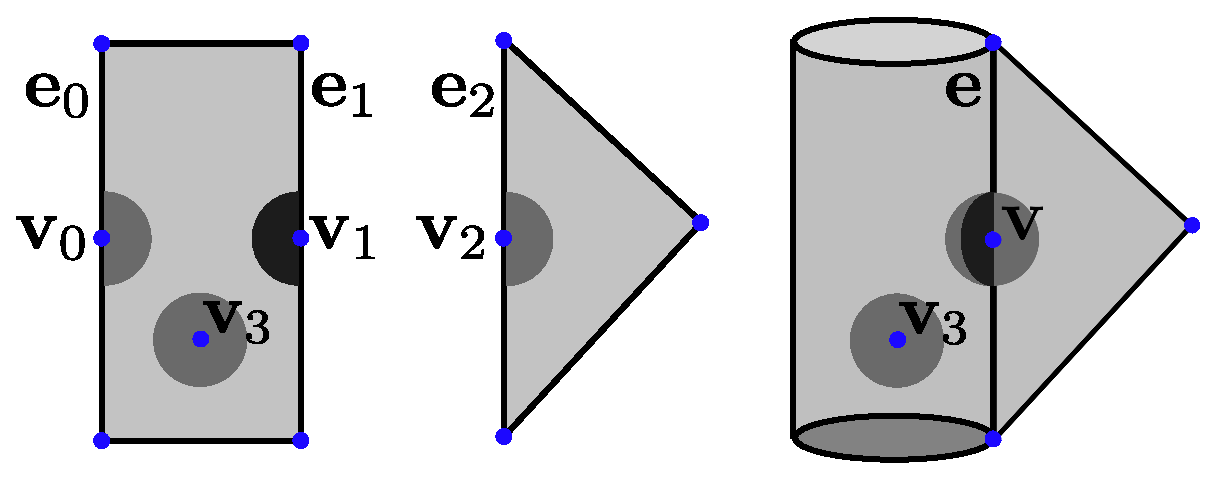
\includegraphics[height=3cm]{screenshots/neighborhood.eps}
\end{center}
\caption{We unify edges $\vec{e}_0$, $\vec{e}_1$ and $\vec{e}_2$, the resulting cell complex or mesh is on the right. The vertex $\vec{v}$ that has been produced by
unifying the other vertices also has a neighborhood that is the result of the unification of $\vec{v}_0$, $\vec{v}_1$ and $\vec{v}_2$ \cite{kinsey1993topology}.}
\label{fig:mesh-neighborhood}
\end{figure}

\end{frame}

\begin{frame}
  \frametitle{Adjacency, Incidence, Valency and Stencil}
From basic graph theory the adjacency and incidency relationships are important for our
considerations:
		\begin{itemize}
			\item \keyword{Adjacency} is the neighborhood relation between same type mesh components whereas \keyword{incidency} is the neighborhood relation between mesh components of
a different type.
			\item Using this terminology we call two polygons adjacent if there is an edge that is incident to both polygons
							 
 
\item The \keyword{stencil} of a vertex is the set of edges and polygons incident to the vertex:
\begin{align*}
  Stencil \text{ } \tau = \{\sigma \in K| \tau < \sigma \}
\end{align*}
\item The \keyword{degree} or \keyword{valency} of a vertex $\vec{v}$ is the number of vertices $\vec{v}_i$ that is adjacent to $\vec{v}$, meaning there exists an edge that connects $\vec{v}$ to $\vec{v}_i$.
\end{itemize}
\end{frame}

\begin{frame}
  \frametitle{Surface Meshes}
\begin{itemize}
\item Usually a triangulation or quadrangulation of a geometric object
\item In CFD simulations used as:
	\begin{itemize}
	  \item Domain boundaries
	  \item Immersed static objects		
	  \item Immersed dynamic objects				
	\end{itemize}
\item Immersion of surface meshes into CFD simulations usually done by \keyword{Fictitious Domain} Methods (FEATFLOW: \keyword{Fictitious Boundary})
\end{itemize}
\begin{figure}[h!]
\centering
\subfloat[Streamline flowfield around a \newline helix geometry]{ 
 \includegraphics[height=3cm]{Images/helix.eps}
 \label{fig:helix}
}%\hspace{0.1cm}
\subfloat[ Twin screw geometry simulation ]{ 
 \includegraphics[height=3cm]{Images/liquidsolid_intro.eps}
 \label{fig:liquidsolid_intro}
}
\caption{CFD Examples with surface meshes}
\label{fig:liquid-solid}
\end{figure}
\end{frame}

\begin{frame}
\frametitle{Surface Meshes Example}

\begin{figure}[h!]
	\begin{center}
	   \includegraphics[width=\textwidth]{screenshots/tori.jpg}
	\end{center}
	%\caption{From left to right: manifold surface, non-manifold at an edge and non-manifold at a vertex.}
	\label{fig:tori}
\end{figure}
\end{frame}

\begin{frame}
For multiple tasks surfaces are required to be \keyword{manifolds}:
\begin{itemize}
\item An $n$-dimensional manifold is a topological space in which every vertex has a neighborhood that is topologically equivalent to an open $n$-dimensional disk. 
\item Two distinct points have disjoint neighborhoods, a surface is a \keyword{2-manifold} 
\item If a manifold has a boundary then there exist vertices that have a neighborhood that is topologically equivalent to an open $n$-dimensional disk or half-disk
\item If a vertex has neither an open disk nor open half-disk neighborhood then it is called \keyword{non-manifold}
\item If a surface has one or more non-manifold vertices then the surface is called a non-manifold surface
\end{itemize}
\begin{figure}[h!]
\begin{center}
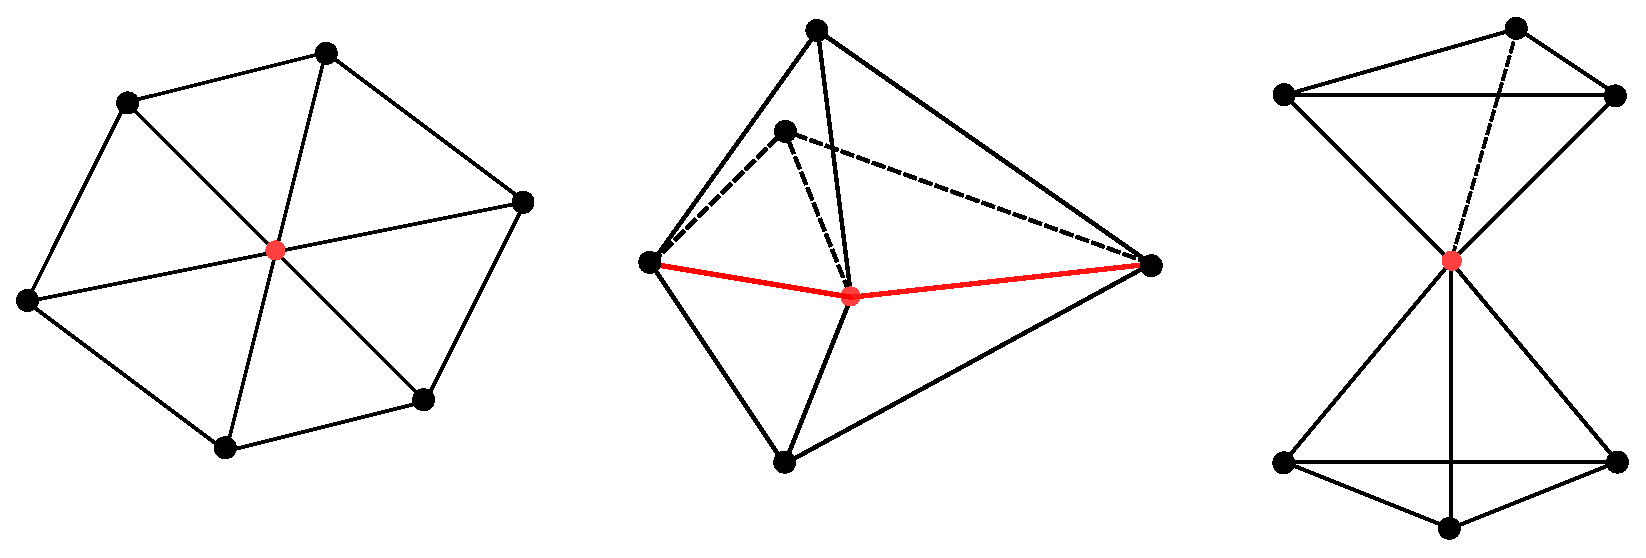
\includegraphics[height=3cm]{screenshots/non_manifolds.eps}
\end{center}
\caption{From left to right: manifold surface, non-manifold at an edge and non-manifold at a vertex.}
\label{fig:non-manifold}
\end{figure}
\end{frame}

\begin{frame}
A bounded manifold can be either \keyword{orientable} or \keyword{non-orientable}
\begin{itemize}
\item A surface is orientable if it does not contain a \keyword{Moebius Strip} \cite{Edelsbrunner:2006:GTM:1137760}.
\item A Moebius Strip can be explained by considering an $(n+1)$-dimensional object moving continiously along an n-manifold
\item If the the object is located on one side of the n-manifold and on its travelling path it revisits a neighborhood, but this time from the other side, then this path is a Moebius Strip and the surface is not orientable
\item The surfaces used to construct two-dimensional meshes are orientable, the cells of these meshes are triangles or quadrilaterals, which are connected by vertices or edges
\item Thus, there should be no isolated vertices or edges that are not part of a polygon in our mesh according to this terminology
\end{itemize}

\begin{figure}[h!]
 \includegraphics[height=3cm]{screenshots/moebius.jpg}
 \label{fig:moebius-render}
\caption{A Moebius Strip can be created by twisting and connecting the edges of a planar strip, see also \cite{Edelsbrunner:2006:GTM:1137760,kinsey1993topology}.}
\label{fig:moebius}
\end{figure}
\end{frame}

\begin{frame}
\frametitle{Software For Generation and Processing of Surface Meshes}

\begin{itemize}
	\item \keyword{Blender}: Creation, manipulation, format conversion, visualization, analysis, postprocessing, open-source, Python scripting
	\item \keyword{Autodesk 3DS Max}: As Blender, but commercial, a bit more advanced manipulation features, proprietary scripting language, Windows only
	\item \keyword{Meshlab}: Mesh analysis, correction of mesh defects, calculation of various mesh properties and indicators
	\item \keyword{Autodesk Inventor}: CAD, creation of meshes from \keyword{NURBS}-Surfaces \cite{NURBSBOOK}
	\item \keyword{FreeCAD}: Open-source CAD program, less functions than Inventor
	\item \keyword{CGAL}: Open-source modern C++ software library for creation, manipulation, analysis, geometric algorithms,...
	\item \keyword{OpenMesh}: Open-source modern C++ data structure for surface meshes from RWTHA 	
\end{itemize}

\end{frame}

\begin{frame}{Data Formats for Surface Meshes}
    \begin{columns}
        \column{0.5\textwidth}{
            \begin{exampleblock}{Element-List}
                \begin{itemize}
                  \item STL
                \end{itemize}
								Properties
                \begin{itemize}
                  \item Stores each element and vertex coordinates
                  \item Redundant repetition of coordinates									
                  \item Problem: Vertex coordinates may not coincide $\rightarrow$ invalid mesh										
                  \item Can store additional properties									
                  \item Main usage for graphics renderings									
                \end{itemize}								
            \end{exampleblock}       }
        \column{0.5\textwidth}{
            \begin{alertblock}{Connectivity-Based}
                \begin{itemize}
                  \item Wavefront OBJ		
                  \item OFF
                  \item Stanford PLY
                  \item VTK									
                \end{itemize}
								Properties:
                \begin{itemize}
                  \item List of vertices, followed by list of elements with vertex indices
									\item more storage efficient
                  \item Some formats allow to store additional properties
                \end{itemize}								
            \end{alertblock}       }
    \end{columns}
\end{frame}

\begin{frame}
\frametitle{OpenMesh - A Surface Mesh Data Structure}
\begin{itemize}
\item \url{https://www.graphics.rwth-aachen.de/software/openmesh/}
\item Uses the efficient halfedge (or winged edge) to the mesh and the connectivity
\item Iterators allow the user to iterate through vertices, edges, faces
\item Circulators allow the user to:
\begin{itemize}
\item iterate over all neighboring vertices of a vertex
\item iterate over all incident edges of a vertex
\item iterate over all faces attached to a vertex
\item iterate over a face's vertices
\item iterate over the face's incident edges
\item iterate over the adjacent faces
\end{itemize}
\item Store user-defined traits in vertices, edges, halfedges, faces	
\item STL-like usage
\end{itemize}								
\end{frame}

\begin{frame}
\frametitle{OpenMesh - The Halfedge Data Structure}
\begin{figure}[h!]
 \includegraphics[width=0.8\textwidth]{screenshots/half-edge.png}
\caption{The OpenMesh Half-Edge Data Structure \cite{Botsch02openmesh}.}
\end{figure}
\end{frame}

\begin{frame}[fragile]

    \begin{lstlisting}[language=C++]
MyMesh mesh;
for(MyMesh::FaceIter f_it = mesh.faces_begin(); f_it != mesh.faces_end(); ++f_it) {
    std::cout << "The face's valence is " 
		          << mesh.valence( *f_it ) 
							<< std::endl;
}\end{lstlisting}     

\begin{lstlisting}[language=C++]
MyMesh mesh;
for (MyMesh::VertexIter v_it=mesh.vertices_sbegin(); v_it!=mesh.vertices_end(); ++v_it) {
  // circulate around the current vertex
  for (MyMesh::VertexVertexIter vv_it=mesh.vv_iter(*v_it); vv_it.is_valid(); ++vv_it)
  {
    // do something with e.g. mesh.point(*vv_it)
  }
}\end{lstlisting}     
\end{frame}

\begin{frame}
%\frametitle{OpenMesh - The Halfedge Data Structure}
\begin{figure}[h!]
 \includegraphics[width=0.8\textwidth]{screenshots/tria-quality.png}
\caption{Triangulations of a Cylinder}
\end{figure}
\end{frame}

\begin{frame}
\frametitle{Meshes for Numerical Simulations}
\begin{itemize}
\item Used to solve discretized PDEs on a computational domain
\item Used i.e. in Finite Volume method (OpenFOAM) and the Finite-Element method
\item Meshes can roughly be grouped into \keyword{structured} and \keyword{unstructured meshes}
\item Meshes need to fulfill quality criteria to facilitate solver convergence
\item Some solvers require special meshes: \keyword{Geometric Multigrid} $\rightarrow$ \keyword{Hierarchical Mesh}
\item Based on the solvers complexity the compute time increases with the degree of mesh refinement (number of elements)
\item \keyword{Domain decomposition} can be used to parallelize the simulation by distributing the subdomains to different processors
\end{itemize}
\end{frame}

\begin{frame}
\frametitle{Structured Meshes}
\begin{itemize}
\item In a structured mesh the valency of every vertices is the same (except for boundary vertices)
\item Consequently, the connectivity is also regular
\item In principle the data structure for a 2D or 3D structured mesh can be a simple 2D or 3D array 
\item Usually not applicable when additional information needs to be stored in the mesh
\item Usual choices of elements in a structured mesh include quadrilateral elements in 2D and hexahedral elements in 3D 
\item Tetrahedrons are possible, but tetrahedrons require more elements to fill a domain with elements
\item Tetrahedrons can represent complex geometries better and automatic mesh generation methods are available
\end{itemize}
\end{frame}

\begin{frame}
There exist different subtypes of structured meshes that are used as computational meshes which mainly include:
\begin{itemize}
\item \keyword{equidistant} cartesian meshes,
\item \keyword{rectilinear} meshes
\item \keyword{curvilinear} meshes 
\end{itemize}
\begin{figure}[h!]
\centering
\subfloat[Equidistant cartesian mesh]{ 
 \includegraphics[height=5cm]{Images/equidistant.eps}
 \label{fig:equidistant}
}\hspace{0.2cm}
\subfloat[Rectilinear mesh]{ 
 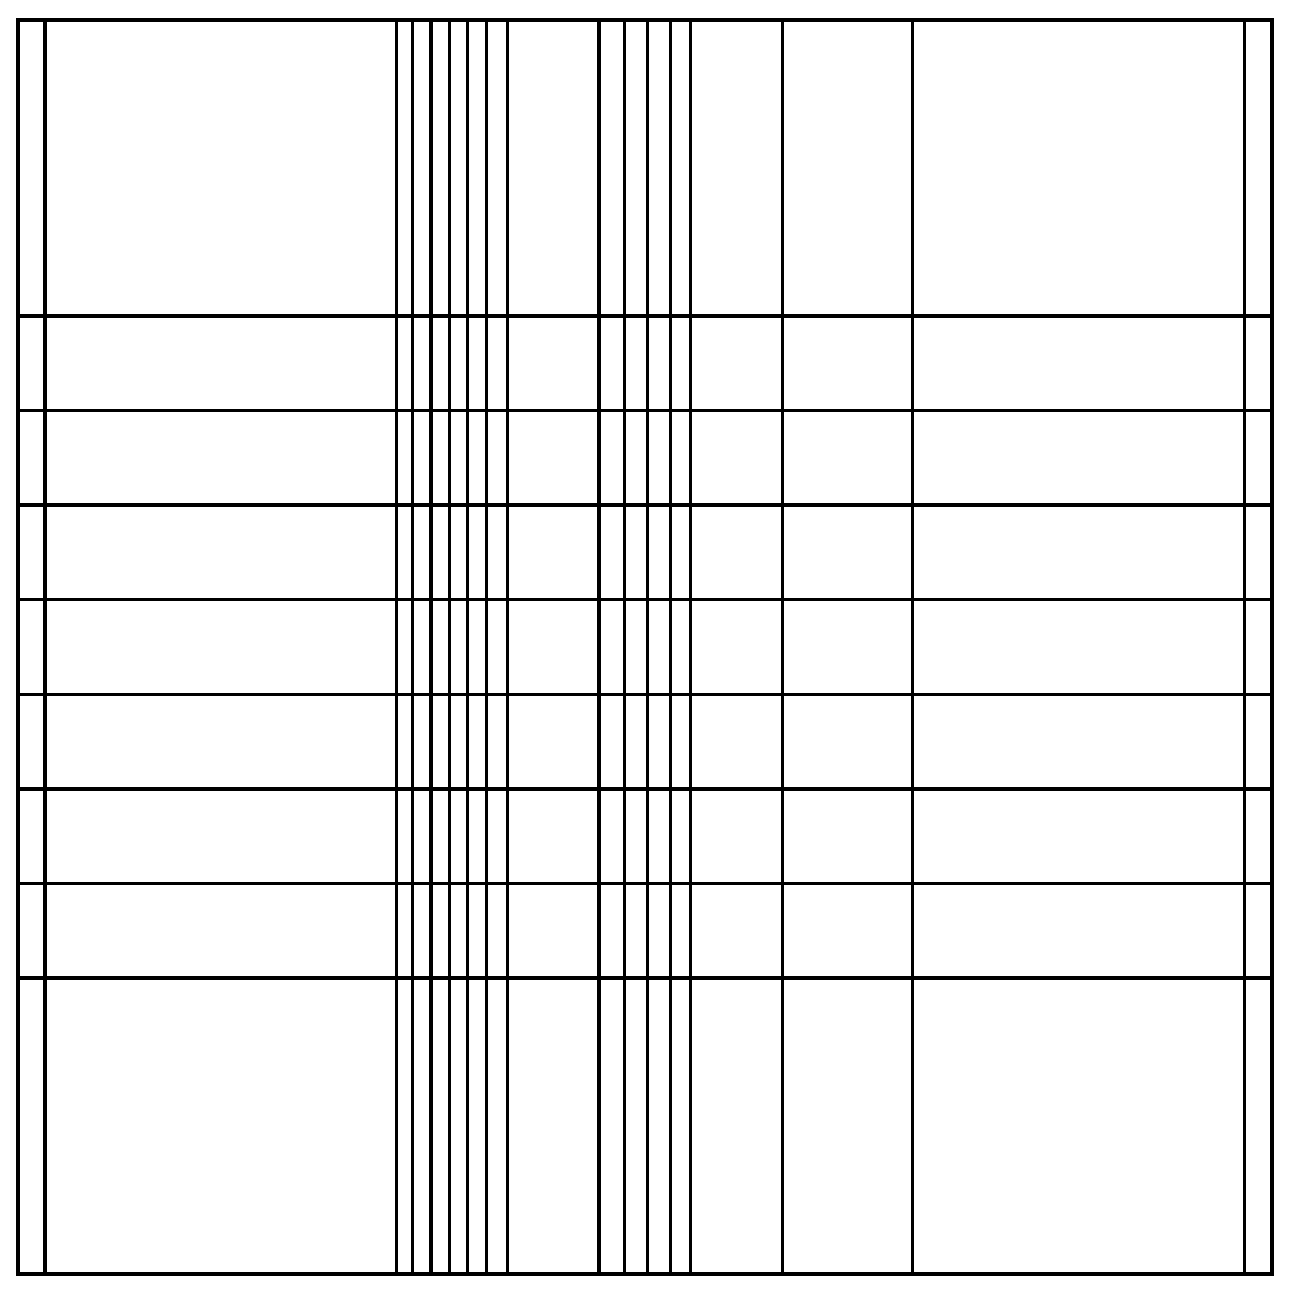
\includegraphics[height=5cm]{Images/rectilinear.eps}
 \label{fig:rectilinear}
}\hspace{0.2cm}
\subfloat[Curvilinear mesh]{ 
 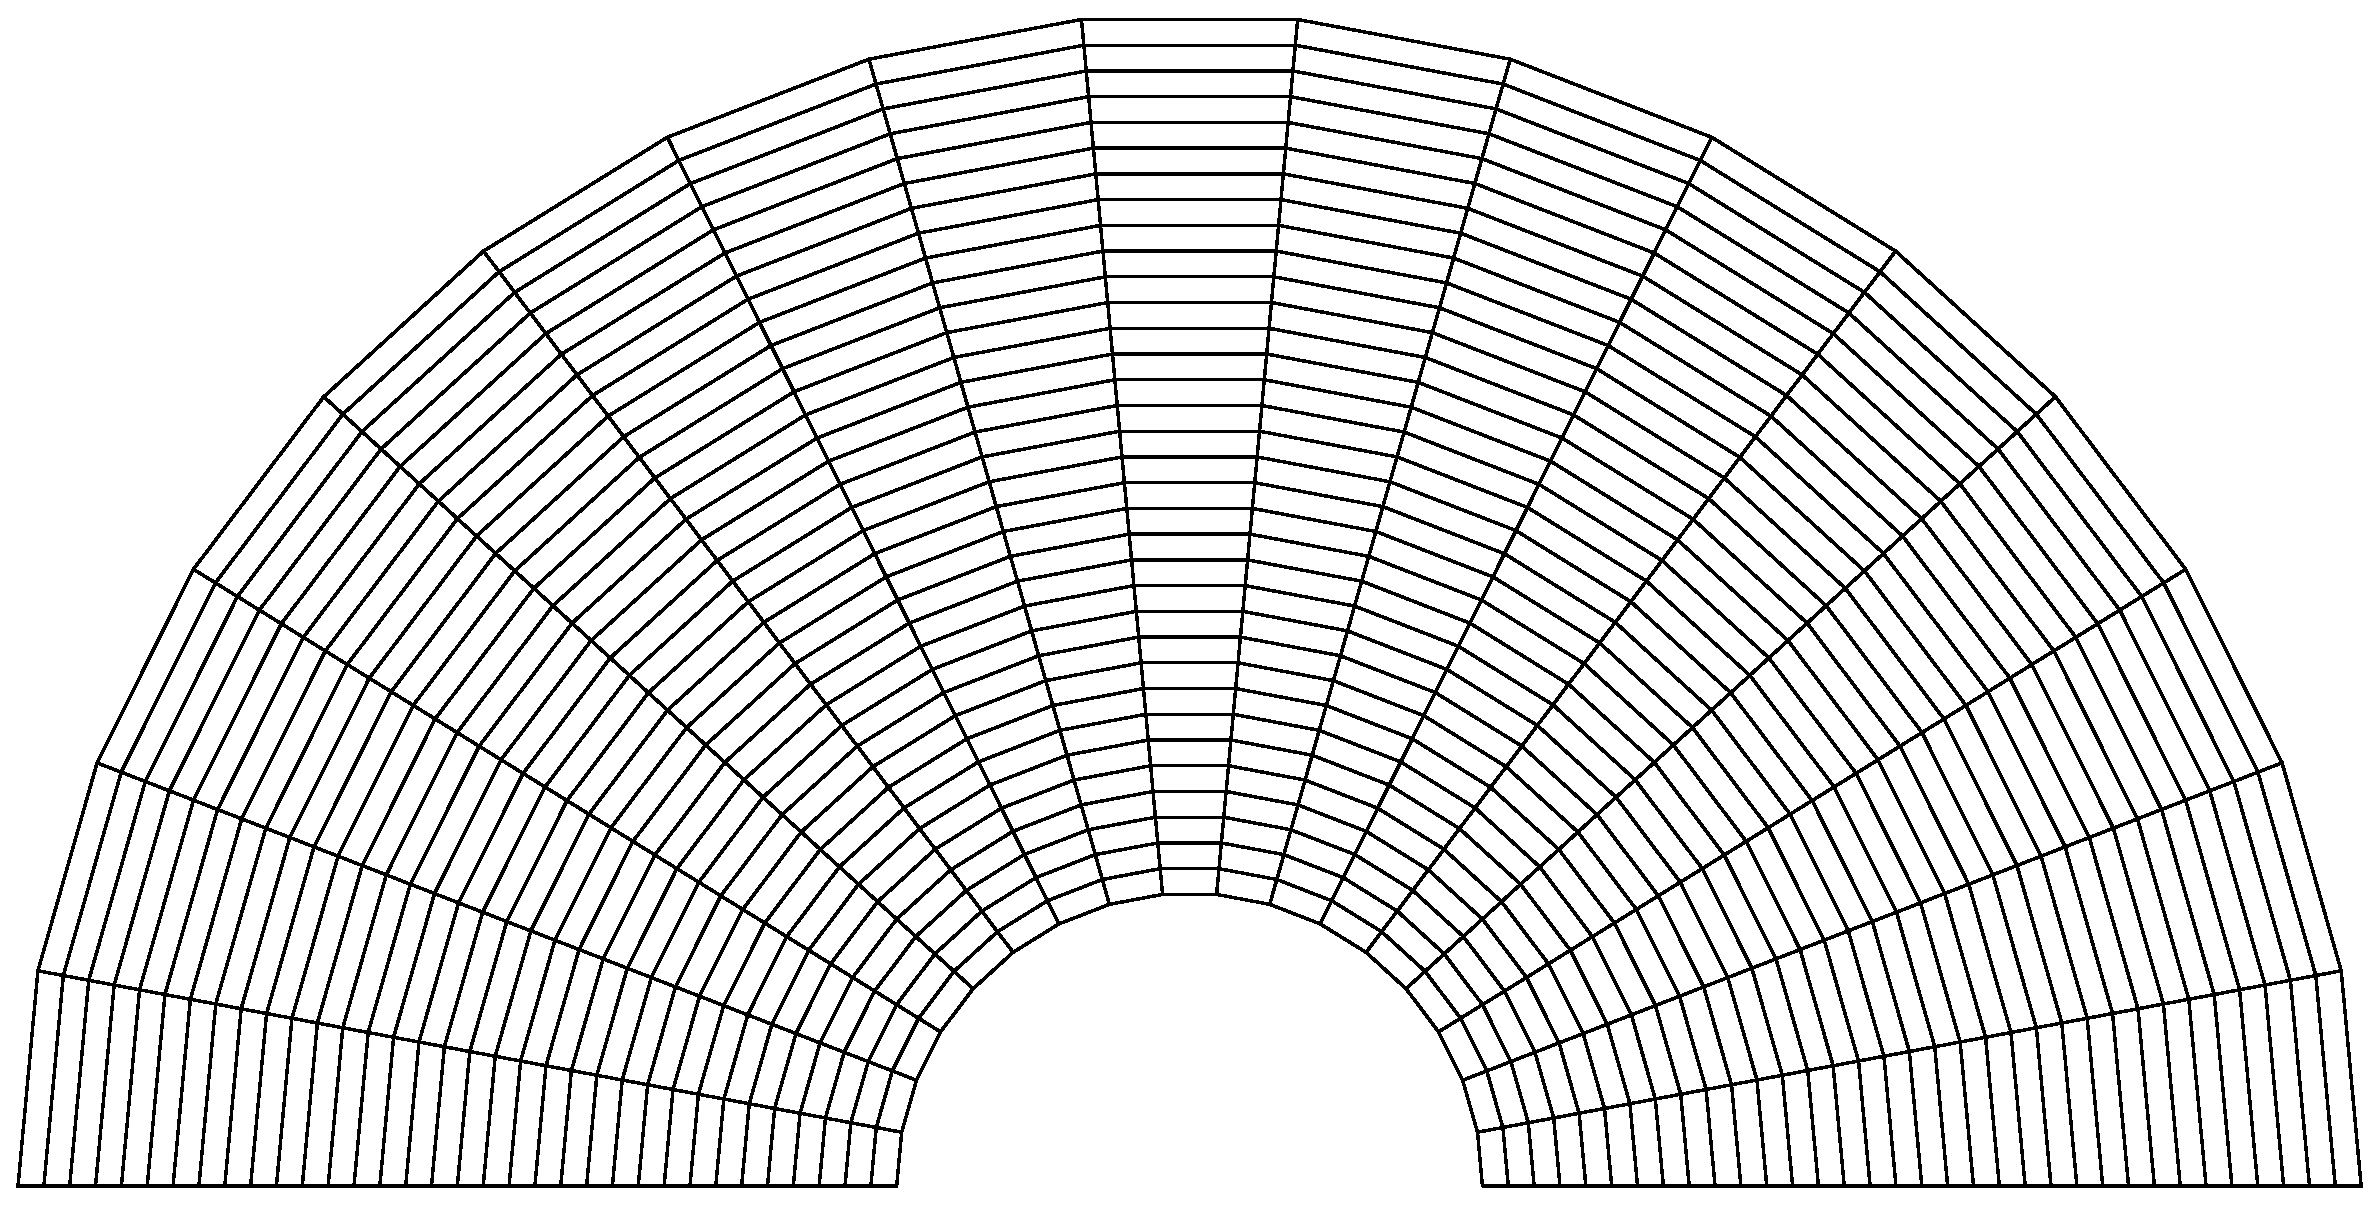
\includegraphics[height=5cm]{Images/curvilinear.eps}
 \label{fig:curvilinear}
}
\caption{Structured meshes used as computational meshes, from left to \\ right: equidistant structured mesh, rectilinear mesh and curvilinear mesh.}
\label{fig:structured}
\end{figure}
\end{frame}

\begin{frame}
\frametitle{Structured Meshes and Point Location}
The equidistant cartesian meshes have an advantageous property: 
\begin{itemize}
\item They have a uniform element size and it is possible to easily locate an arbitrary point in the mesh
\item Useful for many function evaluation tasks
\item Greatly increases computation speed when using immersed geometries and fictious domain/boundary methods
\end{itemize}
For rectilinear and curvilinear meshes this is also possible, but slightly more difficult. In terms of memory representation of such meshes this means that an element index in a data structure can be efficiently computed based on coordinates in space:
\begin{equation*}
  f: \vec{p} \mapsto i\text{ (array index) }, \vec{p} \in \mathbb{R}^3.
  \label{eq:struct-map}
\end{equation*}
\end{frame}

\begin{frame}
\frametitle{Further Advantages of Structured Meshes}
\begin{itemize}
\item Equidistant cartesian meshes are often used for parallel FV, FEM high performance computing schemes
\item Easy generation, memory access patterns and simple domain decomposition
\item Application of equidistant structured meshes as acceleration structures for geometric computations
\item Employed as a means to subdivide space and thus reduce search domain
\item Spatial subdivision structures intended for acceleration of geometric calculations 
\item Example for geometric queries: visibility determination, point containment, distance or intersection queries
\end{itemize}
\end{frame}

\begin{frame}
\frametitle{Unstructured Meshes}
\begin{itemize}
\item In an unstructured mesh the vertices in general do not have a predefined uniform vertex degree
\item In principle this means that an arbitrary number of cells can be incident to a vertex
\item This is helpful for resolving an immersed geometry because edges, faces can be aligned to the shape of the geometry
\item We call these meshes \keyword{aligned unstructured meshes}
\item Better resolution of flow features and geometry increases the accuracy of the result
\item Unstructured meshes can employ connector elements to gradually increase/reduce the level of refinement in a grid
\end{itemize}
\end{frame}

\begin{frame}
\frametitle{Quality Criteria}
The quality of a mesh depends on the quality of its elements. A variety of mesh quality criteria \cite{kellyansys} exist to measure cell quality:
\begin{itemize}
\item Aspect ratio
\item Angle deviation
\item Corner angle
\item Jacobian ration
\item Inverted cells, self-intersecting cells
\end{itemize}
\end{frame}

\begin{frame}
\begin{figure}[h!]
  \centering
  \subfloat[Example of edge length rations]{ 
    \includegraphics[width=0.75\textwidth]{screenshots/edge-ratio.jpg}
    \label{fig:edgeration}
  }\\
  \subfloat[Examples of angle deviation values]{ 
    \includegraphics[width=0.75\textwidth]{screenshots/angle-deviation.jpg}
    \label{fig:angledev}
  } 
\end{figure}
\end{frame}

\begin{frame}
\begin{figure}[h!]
  \centering
  \subfloat[Maximum inner angle criterium]{ 
    \includegraphics[width=0.75\textwidth]{screenshots/inner-angle.jpg}
    \label{fig:innerangle}
  }\\
  \subfloat[Examples of angle deviation values]{ 
    \includegraphics[width=0.75\textwidth]{screenshots/jacobi-deviation.jpg}
    \label{fig:jacobideviation}
  } 
\end{figure}
\end{frame}

\begin{frame}
\begin{figure}[h!]
  \centering  
    \includegraphics[width=0.75\textwidth]{screenshots/inversion.jpg}
		\caption{Cell self-intersection, inverted cell}
  \label{fig:camaro-mesh}
\end{figure}
\end{frame}

\begin{frame}
\frametitle{Embedding Geometries with the Fictitious Boundary Method}
\begin{itemize}
\item Unstructured meshes in order to better approximate complex-shaped geometries introduces some difficulties as well
\item For Fictitious Boundary type methods one has to know which vertices of the mesh are solid vertices and which are fluid vertices
\item In order to set appropriate boundary conditions an inside/outside indicator function has to be computed
\end{itemize}
\begin{equation*}
 \alpha_{i} (\vec{x}) = 
   \begin{cases}1  &  \mbox{for } \vec{x} \in \Omega_{s}, \\
                0  &  \mbox{for } \vec{x} \in \Omega_{f} \setminus \Omega_s  
   \end{cases}   
\end{equation*}
\begin{itemize}
\item $\Omega_{s}$: solid domain
\item $\Omega_{f}$: fluid domain
\end{itemize}
\end{frame}

%domain areas where a high mesh resolution is required to domain areas where such a high mesh resolution is not needed (see figure \ref{fig:unstructured-fac}). This property is a %clear advantage over structured meshes where the mesh resolution can only be increased globally or by local vertex redistribution without changing the 
%connectivity of the mesh. The . Complex 
%geometries are often explicitly defined by a set of coordinates in space or by an explicit or implicit analytic function. Using an unstructured mesh there is 
%in general no easy way to introduce a mapping from positions in space to element indices in computer memory. Which means that calculations that involve geometric 
%information about the object that is represented by the mesh may need to resort to exhaustive search procedures if no measure are taken to add this feature to the 
%class of unstructured meshes. Possible solutions to this problem are discussed in the following chapters. Standard choices for cell geometries in unstructured meshes are hexahedrons, tetrahedrons or prisms.\\

\begin{frame}
\begin{figure}[h!]
\begin{center}
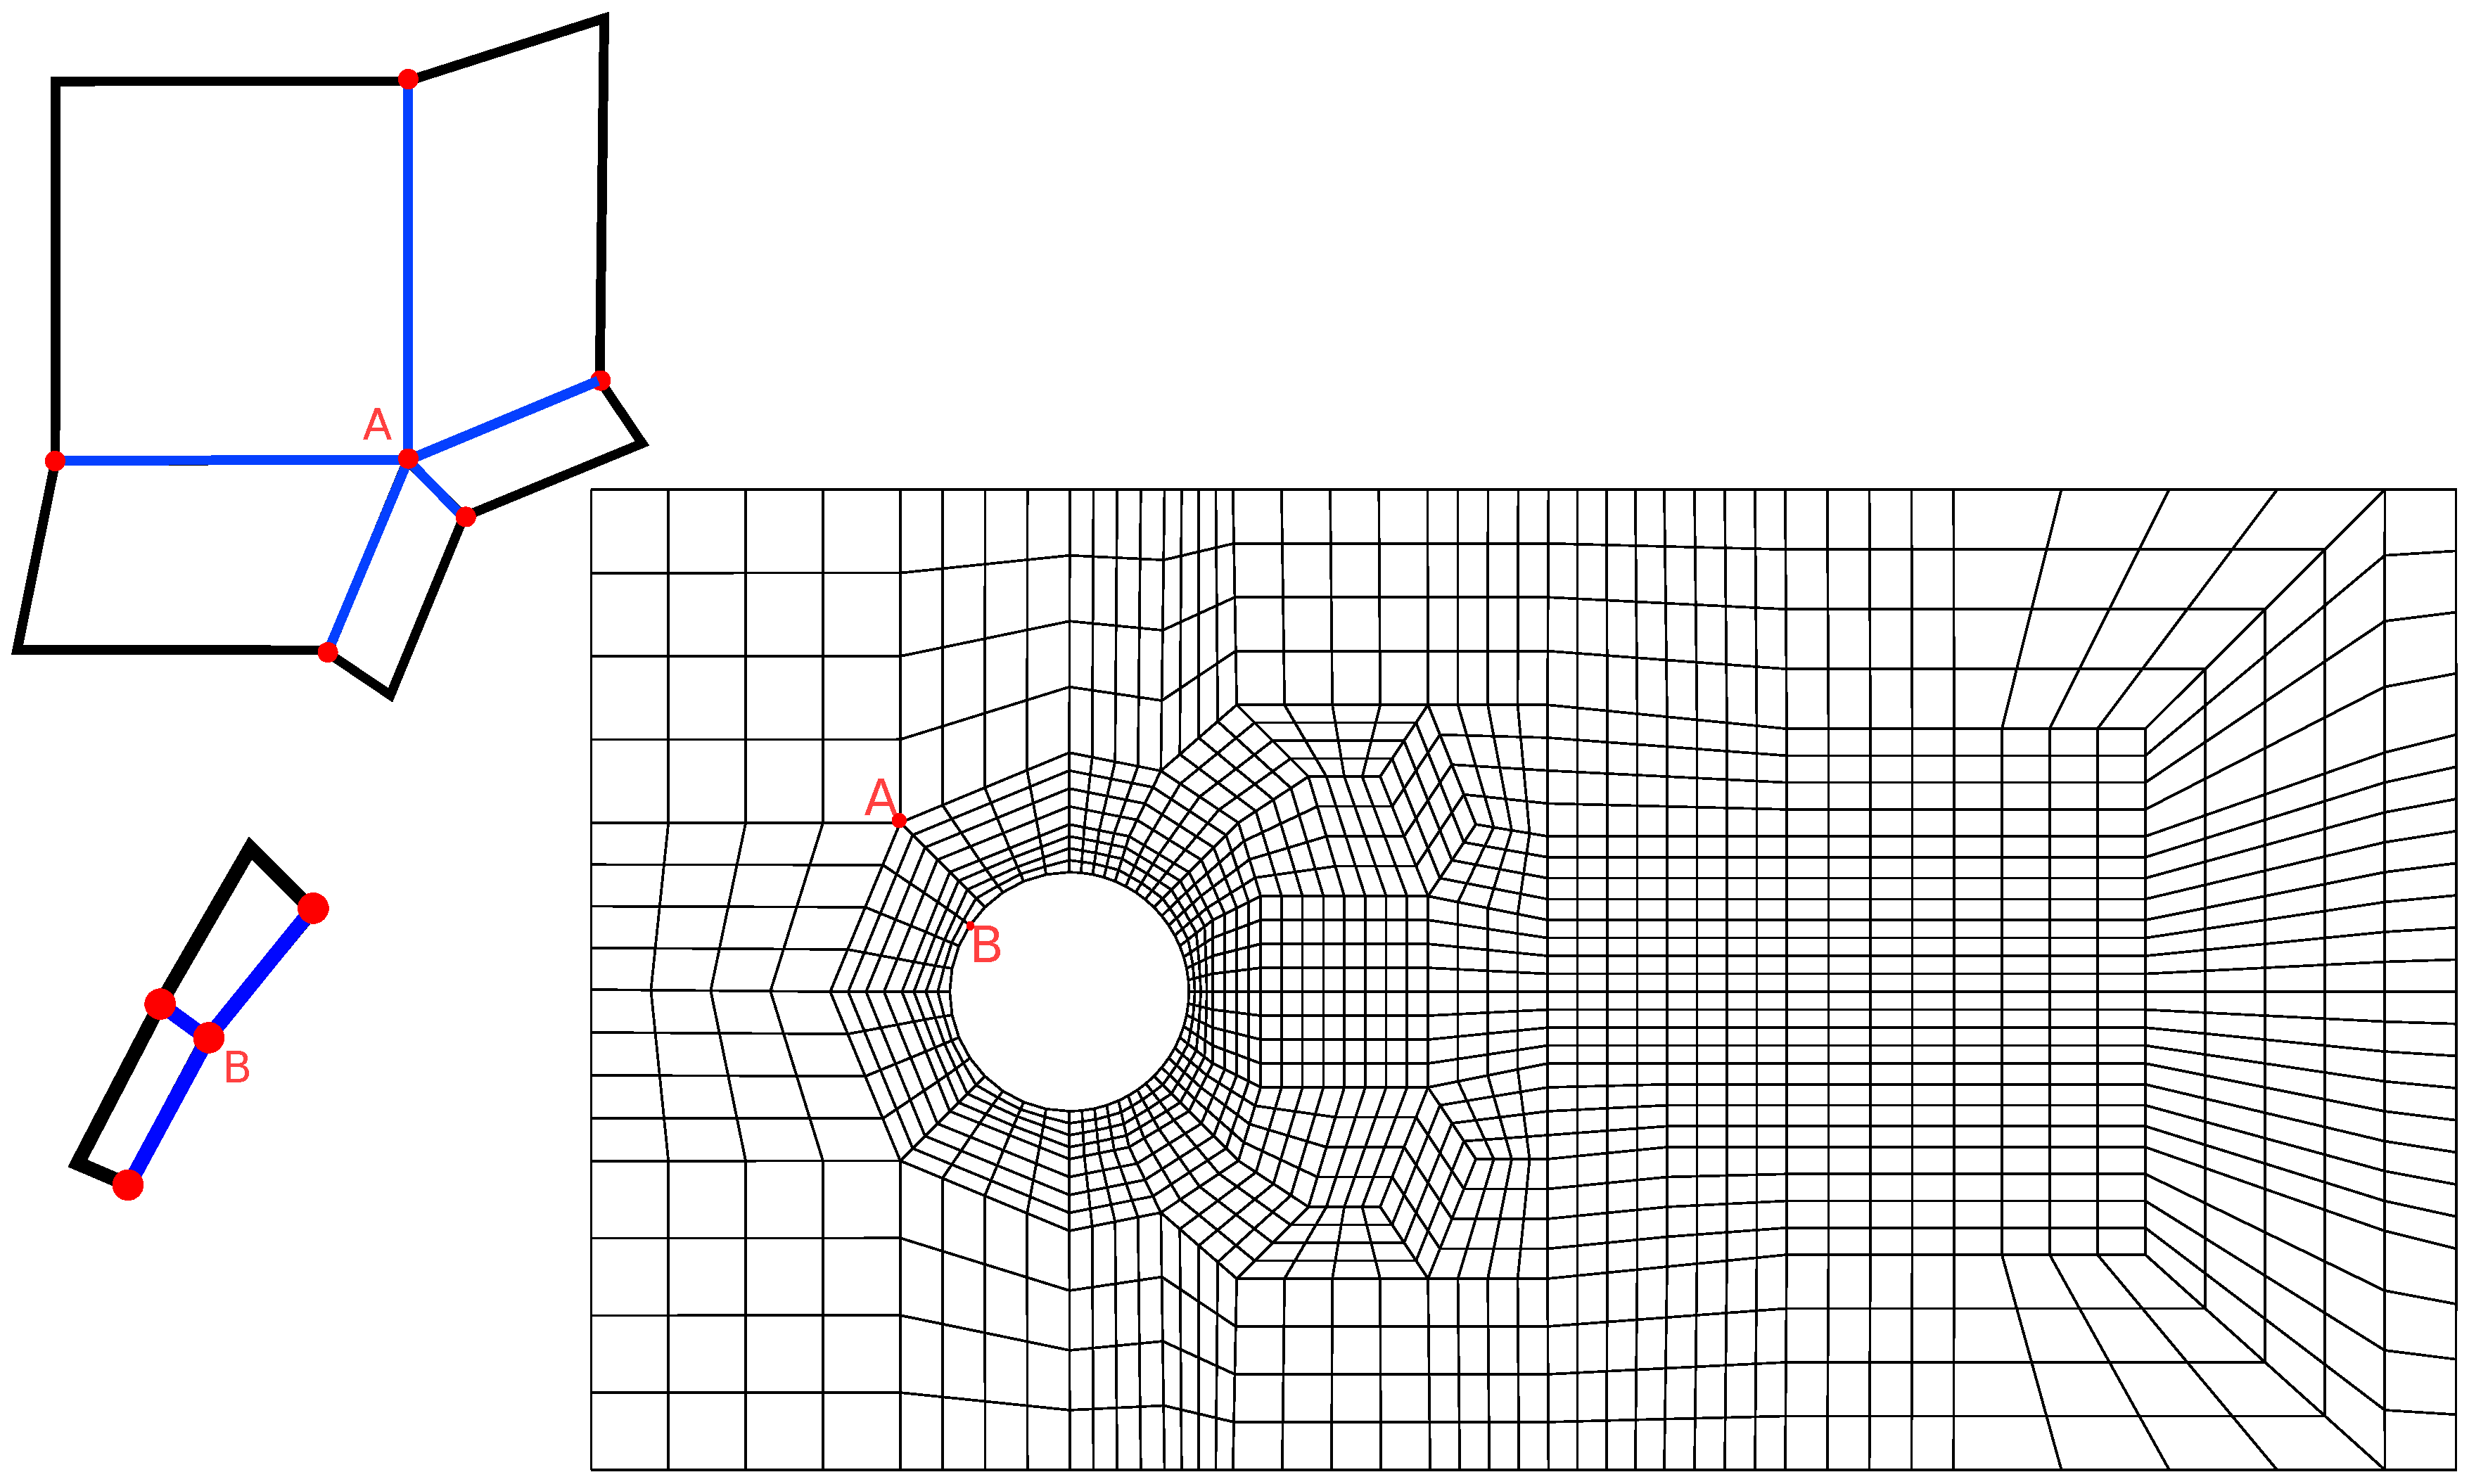
\includegraphics[width=0.7\textwidth]{Images/fac_unstructured.eps}
\end{center}
\caption{Unstructured 2D mesh where the mesh edges are aligned with an inner circle. We have marked some vertices with different 
degrees to that are used as anchor for connector elements (A) or as elements that approximate the circle geometry with its edges (B).}
\label{fig:unstructured-fac}
\end{figure}
\end{frame}

\begin{frame}
\begin{figure}[h!]
  \centering
  \subfloat[Mesh view with indicator function]{ 
    \includegraphics[width=0.5\textwidth]{Images/car.eps}
    \label{fig:camaro-nondef}
  }
  \subfloat[Rendered surface mesh of the geometry]{ 
    \includegraphics[width=0.5\textwidth]{Images/camaro.eps}
    \label{fig:camaro}
  }
  \caption{Inside/outside indicator function}
  \label{fig:camaro-mesh}
\end{figure}
\end{frame}

\begin{frame}
\frametitle{Data Structures for Unstructured Meshes}
\begin{itemize}
\item Data structure needs to support hierarchical meshes/mesh levels $\rightarrow$ multi-grid solver
\item FEATFLOW based or derived software packages use the two-level ordering
\item Lowest Mesh level called the coarse grid
\item Mesh levels build successively, during refinement append vertices of next mesh level at the end of the vertex array
\item Thus indices in the connectivity information remain valid during refinement
\item Store connectivity arrays for each level individually
\end{itemize}
\end{frame}

\begin{frame}
\begin{figure}[h!]
\centering
\subfloat[The coarse mesh] {
\centering
 \includegraphics[width=0.35\textwidth]{Images/tc_base_mesh.eps}
 \label{fig:tc_base_mesh}
}
\hspace{1.0cm}
\subfloat[The fine mesh] {
\centering
 \includegraphics[width=0.35\textwidth]{Images/tc_mesh.eps}
 \label{fig:tc_mesh}
}
\caption{Pre-adapted hierachical mesh}
\label{fig:bench_setup}
\end{figure}
\end{frame}

\begin{frame}[fragile]
\frametitle{Unstructured Meshes Two-Level Ordering (FEATFLOW)}
\begin{itemize}
\item NVT: number of vertices on a level
\item NMT: number of edges on a level
\item NAT: number of faces on a level
\item NEL: number of faces on a level
\item During regular refinement we generate NMT+NAT+NEL new vertices
\item These are stored at the end of the current vertex array with the corresponding indices
\end{itemize}
Example of a 2D vertex array after a regular refinement. Before the refinement the length of the vertex array is NVT:
\begin{tikzpicture}
\matrix (A) [matrix of nodes,
                       every node/.style={text depth=.5ex,text height=2ex},
                       nodes={draw, minimum size=8mm, anchor=center}, 
											 nodes in empty cells, minimum height = 2cm,
											 row 2/.style={nodes={draw=none}},
											 row 3/.style={nodes={draw=none}},column sep=-\pgflinewidth,]											
    {		 
		 v & $\dots$ & v & e & $\dots$ & e & c & \dots & c\\
		$\uparrow$ & $\uparrow$ & $\uparrow$ & $\uparrow$ & $\uparrow$ & $\uparrow$ & $\uparrow$  & $\uparrow$ & $\uparrow$\\
		1 &  & nvt & nvt+1 &  & nvt+nmt & nvt+nmt+1 & & nvt+nel\\		
		};
%\foreach \i [evaluate=\i as \ni using {int(\i)}, evaluate=\i as \ntext using {int(\i)}] in {1,3,4,6} 
%    \draw [{Stealth}-, red!70] (A-1-\ni.south west)--++(-90:5mm) node[below] {\ntext};
\end{tikzpicture}
\end{frame}

\begin{frame}
\frametitle{Domain Decomposition}
\begin{figure}[h!]
\centering
\includegraphics[height=7cm]{Images/domains.eps}
\caption{Domain Decomposition in FEATFLOW: Whole domain (left), domain decomposed in 4 subdomains (right)}
\label{fig:domains}
\end{figure}
\end{frame}

\begin{frame}
\frametitle{Domain Decomposition for HPC}
\begin{itemize}
\item Solve the problem on the whole domain by computing a partial solution on each \keyword{subdomain}
\item The partial solutions on the subdomain are computed by different processing cores
\item \keyword{Domain Decomposition}: decompose or partition the domain into 'equal' subdomains
\item The amount of work that is assigned to each core should be as equal as possible
\item The amount of communication between cores/subdomains should be minimal
\item Software libraries for domain decomposition: 
\begin{itemize}
\item \keyword{Metis}: \url{http://glaros.dtc.umn.edu/gkhome/views/metis/}, FEATFLOW
\item \keyword{Scotch}: \url{https://www.labri.fr/perso/pelegrin/scotch/}, OpenFOAM
\end{itemize}
\end{itemize}
\end{frame}

\begin{frame}
\frametitle{Graph Theory and Domain Decomposition}
\begin{itemize}
%\item In the simulation workflow domain decomposition follows grid generation
\item Domain decomposition libraries such as Metis/Scotch use \keyword{Graph Theory} for decomposition
\item Meshes/Matrices can be represented as Graphs (i.e. Undirected Graph and Adjacency Matrix)
\item Graph Theory is also used for sparse matrix reordering 
\item The class of algorithms used in domain decomposition is \keyword{Graph Partitioning} algorithms
\item Graph partitioning algorithms can on their own be executed in parallel
\end{itemize}
\begin{figure}[h!]
\centering
\includegraphics[height=5cm]{screenshots/domain-decomposition.png}
\label{fig:domains}
\end{figure}
\end{frame}

\begin{frame}
\frametitle{Mesh Adaptivity/Deformation}
\begin{itemize}
\item Accuracy of the simulation result increases with mesh resolution
\item Often a high accuracy solution is needed most in certain areas of interest
\item \keyword{Mesh adaptation} is used to increase mesh resolution without regular refinement
\item Different approaches to mesh adaptivity exist (some create \keyword{hanging nodes})
\item In \keyword{h-adaptivity} cells in a region of interest of the mesh are locally refined
\item The mesh connectivity is changed in the h-adaptivity approach
\item Hanging nodes can be a avoided by using connector elements
\item \keyword{r-adaptivity} moves existing nodes to increase resolution in regions of interest
\end{itemize}
\end{frame}

\begin{frame}
\begin{figure}[h!]
\centering
\subfloat[Adaptation to a circle by r-adaptivity] { 
 \includegraphics[width=10cm]{Images/fbm_r_adapt.eps}
}\\
\subfloat[Mesh adaptation to an airfoil by h-adaptivity] { 
 \includegraphics[width=10cm]{Images/h-adapt.eps}
}
\caption{Different types of mesh adaptation}
\end{figure}
\end{frame}

\begin{frame}
\frametitle{Local Refinement with Connector Elements}
\begin{figure}[h!]
\centering
\includegraphics[width=0.48\textwidth]{screenshots/PROTOTYPE2.png}
\caption{Courtesy O.Mierka}
\label{fig:domains}
\end{figure}
\end{frame}

\begin{frame}
\begin{figure}[h!]
\centering
\includegraphics[width=0.5\textwidth]{screenshots/P4.png}
\label{fig:domains}
\caption{Courtesy O.Mierka}
\end{figure}
\end{frame}

\begin{frame}
\begin{figure}[h!]
\centering
\includegraphics[width=1.\textwidth]{screenshots/GEO_BIW.png}
\label{fig:domains}
\caption{Courtesy O.Mierka}
\end{figure}
\end{frame}

\begin{frame}
\frametitle{R-Adaptivity}
\begin{itemize}
\item Moves existing nodes into region of interest without changing mesh connectivity
\item The r-adaptivity approach usually uses a \keyword{monitor function} to prescribe where nodes should be moved
\item The monitor function often uses distance calculations to move nodes that are already close to the region of interest
\item R-adaptivity can produce invalid elements (i.e. self-intersections) 
\item Iterative movement of nodes with smoothing passes can help prevent invalid elements
\item There exist PDE-based approaches \cite{GrajewskiKoesterTurek2008b} for r-adaptivity and algebraic methods based on \keyword{Laplacian Smoothing} \cite{Muenster:2016}
\end{itemize}
\end{frame}

\begin{frame}
\frametitle{Algebraic Mesh Adaptation using weighted Laplacian Smoothing}
\keyword{Laplacian smoothing} is usually used on meshes to reduce noise, it tries to rearrange nodes more to the center of its surrounding nodes. Laplacian smoothing in its smoother form is represented by the following equation:
\begin{equation*}
\mathbf{x}_{new} = (1-\omega) \cdot \mathbf{x} + \frac{\omega}{{\rm e}(\mathbf{x})} \cdot \sum\limits_{j=1}^{{\rm e}(\mathbf{x})} \mathbf{x}_j, 
\label{eq:laplace-smoother}
\end{equation*}
We can introduce vertex weights in order to move vertices closer to the region of interest, be giving vertices in that region a higher weight:
\begin{equation*}
\mathbf{x}_{i}^{\rm new} = (1-\omega) \cdot \mathbf{x}_{i}^{\rm old} + \omega \cdot \frac{\sum\limits_{j=1,n}^{{{\rm e}(i)}} w_j \mathbf{x}_j^{\rm old}}{\sum\limits_{j=1}^{{\rm e}(i)} w_j}\quad {\rm for} \quad i=1,n
\end{equation*}
\end{frame}

\begin{frame}
\begin{figure}[h!]
\centering
\subfloat[The weights for the laplace smoother are generated by combining the signed distance $d(\mathbf{x})$ with a hat function] { 
 \includegraphics[width=10cm]{Images/monitor_func.eps}
 \label{fig:mon}
}\hspace{0.1cm}
\subfloat[Visualization of $w(\mathbf{x})$ on the undeformed mesh] {
  \raisebox{3.5\baselineskip}{
 \includegraphics[width=10cm]{Images/mon}
 \label{fig:mon_field}
 }
}
\caption{Generation of the weight distribution function $w(\mathbf{x})$}
\label{fig:monitor_func}
\end{figure}

\end{frame}

\begin{frame}[plain]
\begin{figure}[h!]
  \centering
  \subfloat[Cylinder appears round in a two-color map]{ 
    \includegraphics[width=13.0cm]{Images/fbm_laplace_con.eps}
  }\\
  \subfloat[The mesh nodes are concentrated near the surface of the cylinder]{ 
    \includegraphics[width=13.0cm]{Images/fbm_laplace_con_edges.eps}
  }
  \caption{Cylinder resolution for the Laplace-$\kappa$ adaptation}
  \label{fig:osc-cyl-lap-kappa}
\end{figure}
\end{frame}

\begin{frame}[plain]
\begin{figure}[h!]
  \begin{center}
    \includegraphics[width=1.0\textwidth]{Images/drag_coefficient_laplace_kappa_classic_fbm.eps}
    \caption{Drag curves for the standard FBM, Laplace-$\alpha$ and Laplace-$\kappa$ calculations}
    \label{fig:drag-kappa-classic}
  \end{center}
\end{figure}
\end{frame}

\begin{frame}[plain]
\begin{figure}[h!]
  \begin{center}
    \includegraphics[width=1.0\textwidth]{Images/lift_kappa_fbm.eps}
    \caption{Drag curves for the standard FBM, Laplace-$\alpha$ and Laplace-$\kappa$ calculations}
    \label{fig:lift-kappa-classic}
  \end{center}
\end{figure}
\end{frame}

\begin{frame}
\frametitle{Mesh Generator Salome}
\begin{itemize}
\item \url{https://www.salome-platform.org/}
\item Full-featured open-source CAD + mesh generator 
\item Integrates many open-source meshing libraries by plug-ins (i.e. netgen)
\item Allows a user to design geometries with semantic parts (inflow, outflow, walls, ...)
\item Calculate quality metrics on meshes
\item Many different mesh format available (i.e., export to OpenFOAM)
\item Possible to execute tasks in batch mode by Python scripts
\item Geared towards students, good documentation and example projects
\end{itemize}
\end{frame}

